% Créé le 01/10/2020 Thu 13:00 
\documentclass[10pt]{article}

\usepackage[defaultfam,light,tabular,lining]{montserrat} %% Option 'defaultfam'
%% only if the base font of the document is to be sans serig
\renewcommand*\oldstylenums[1]{{\fontfamily{Montserrat-TOsF}\selectfont #1}}

\RequirePackage[utf8]{inputenc}
\RequirePackage[T1]{fontenc}

\RequirePackage{setspace}              %%pour le titre
\RequirePackage{graphicx}	        %% gestion des images
\RequirePackage[dvipsnames,table]{xcolor}	%% gestion des couleurs
\RequirePackage{array}		%% gestion améliorée des tableaux
\RequirePackage{calc}		        %% syntaxe naturelle pour les calculs
\RequirePackage{enumitem}	        %% pour les listes numérotées
\RequirePackage[footnote]{snotez}	%% placer les notes de pied de page sur le coté
\RequirePackage{microtype,textcase}
\RequirePackage{titlesec}
\RequirePackage{booktabs}

\RequirePackage{amsmath,
	amssymb,
	amsthm} 			%% For including math equations, theorems, symbols, etc
\RequirePackage[toc]{multitoc}

\RequirePackage[a4paper,left=15mm,
top=15mm,headsep=2\baselineskip,
textwidth=132mm,marginparsep=8mm,
marginparwidth=40mm,textheight=58\baselineskip,
headheight=\baselineskip]{geometry}

\microtypesetup{protrusion=true,final}
%%----------------------------------------------------------------------------------------
%%	HEADERS
%%----------------------------------------------------------------------------------------
\makeatletter

\newenvironment{fullpage}
    {\skip\noindent\begin{minipage}
    {\textwidth+\marginparwidth+\marginparsep}\skip\smallskip}
    {\end{minipage}
%%\vspace{2mm}
}


%% COLOR %<--------------------------------------------------------->%
\RequirePackage{xcolor}

%% Contrast colours
\definecolor{mdgreen}{HTML}{A4C21F}

%% Additional colours
\definecolor{mdgrey}{HTML}{A19589}
\colorlet{mdgray}{mdgrey}
\definecolor{mdlightgrey}{HTML}{D8D0C7}
\colorlet{mdlightgray}{mdlightgrey}


%% DOC %<----------------------------------------------------------->%

\ProcessOptions\relax

%% Command to provide alternative translations in French and English
\newcommand{\FrenchEnglish}[2]{
   \iflanguage{french}{#1}{}
   \iflanguage{english}{#2}{}}

%% This} separating line is used across several documents,
\newcommand{\@separator}{%%
 %% To make sure we have spacing on both sides, make an invisible rule, 2X tall
  \rule{0ex}{2ex}%%
   %% Place the dashed rule 1X high
  \textcolor{mdgray}{\rule[1ex]{\textwidth}{0.25pt}}%%
}


%% LABEL %<-------------------------------------------------------->%
%% Standard style for labels, small and bold
\newcommand{\@labeltext}{\large\scshape}

\newcommand*{\@approvedlabel}{\FrenchEnglish{APPROUVE PAR}{APPROVED BY}}
\newcommand*{\@approved}{Set with \texttt{	extbackslash approved\{\}}}
\newcommand*{\approved}{\renewcommand*{\@approved}}

\newcommand*{\@authorlabel}{\FrenchEnglish{Auteur(s)}{Author(s)}}
\newcommand*{\@Authorlabel}{\FrenchEnglish{AUTEUR(S)}{AUTHOR(S)}}

\newcommand*{\@checkedlabel}{\FrenchEnglish{VERIFIE PAR}{CHECKED BY}}
\newcommand*{\@checked}{Set with \texttt{	extbackslash checked\{\}}}
\newcommand*{\checked}{\renewcommand*{\@checked}}

\newcommand*{\@datelabel}{\FrenchEnglish{DATE}{DATE}}
\newcommand*{\@absentlabel}{\FrenchEnglish{ABSENT}{ABSENT}}
\newcommand*{\@excusedlabel}{\FrenchEnglish{EXCUSE}{EXCUSED}}

\newcommand*{\@durationlabel}{\FrenchEnglish{DUREE}{DURATION}}
\newcommand*{\@duration}{Set with \texttt{\textbackslash duration\{\}}}
\newcommand*{\duration}{\renewcommand*{\@duration}}

\newcommand*{\@initiatorlabel}{\FrenchEnglish{INITIATEUR}{INITIATED BY}}
\newcommand*{\@initiator}{Set with \texttt{\textbackslash initiator\{\}}}
\newcommand*{\initiator}{\renewcommand*{\@initiator}}

\newcommand*{\@participantlabel}{\FrenchEnglish{PARTICIPANT}{PARTICIPANT}}
\newcommand*{\@participantslabel}{\FrenchEnglish{PARTICIPANTS}{PARTICIPANTS}}

\newcommand*{\@preparedlabel}{\FrenchEnglish{PREPARE PAR}{PREPARED BY}}
\newcommand*{\@prepared}{Set with \texttt{\textbackslash prepared\{\}}}
\newcommand*{\prepared}{\renewcommand*{\@prepared}}

\newcommand*{\@presentlabel}{\FrenchEnglish{PRESENT}{PRESENT}}

\newcommand*{\@projectlabel}{\FrenchEnglish{PROJET}{PROJECT}}
\newcommand*{\@project}{Set with \texttt{\textbackslash project\{\}}}
\newcommand*{\project}{\renewcommand*{\@project}}

\newcommand*{\@referencelabel}{\FrenchEnglish{REFERENCE}{REFERENCE}}

\newcommand*{\@reportlabel}{\FrenchEnglish{Rapport}{Report}}

\newcommand*{\@reportnumberlabel}{\FrenchEnglish{RAPPORT N°}{REPORT NUMBER}}
\newcommand*{\@reportnumber}{Set with \texttt{\textbackslash reportnumber\{\}}}
\newcommand*{\reportnumber}{\renewcommand*{\@reportnumber}}

\newcommand*{\@wheremeeting}{Set with \texttt{\textbackslash wheremeeting\{\}}}
\newcommand*{\wheremeeting}{\renewcommand*{\@wheremeeting}}

\newcommand*{\@whenmeeting}{Set with \texttt{\textbackslash whenmeeting\{\}}}
\newcommand*{\whenmeeting}{\renewcommand*{\@whenmeeting}}


%% TASKS

\newcommand*{\@tasklistlabel}{\FrenchEnglish{Liste de tâches}{Task List}}
\newcommand*{\@tasknumberlabel}{\#}
\newcommand*{\@tasklabel}{\FrenchEnglish{TACHE}{TASK}}

\newcommand*{\@duelabel}{\FrenchEnglish{DATE D'ECHEANCE}{DUE DATE}}

\newcommand*{\@responsiblelabel}{\FrenchEnglish{RESPONSABLE}{RESPONSIBLE}}


%% MINUTES %<------------------------------------------------------->%
\ProcessOptions\relax

\PassOptionsToPackage{table}{xcolor}

\renewcommand*{\@authorlabel}{\FrenchEnglish{ECRIT PAR}{WRITTEN BY}}


%% Setting up header and footer
\RequirePackage{nccfancyhdr,lastpage}
\pagestyle{fancy}

%% Header
\renewcommand{\headrulewidth}{0pt}

%% Footer
\renewcommand{\footrulewidth}{0pt}
\fancyfoot[c]{%%
  \sffamily%%
  \color{mdgray}
  \@separator\newline
  ~~%%
  \begin{minipage}[c]{0.5\textwidth}
    \hspace*{3pt}\small{\textbf{\@projectlabel}}\newline
    \hspace*{\tabcolsep}\@project
  \end{minipage}%%
  \hfill
  \thepage\ \FrenchEnglish{de}{of} \pageref{LastPage}
  ~~\newline
  \@separator
}



%% The logo box.
\newcommand{\@rlogo}{
  \noindent
  \scriptsize
  \raggedleft
  \setlength{\parskip}{1ex}
  \includegraphics[height=70px,width=70px,keepaspectratio]{\@mainlogo}
%%\includegraphics[width=\textwidth]{\@mainlogo}
}


\RequirePackage{xparse}
\newcommand{\@participantstable}{}
\NewDocumentCommand \participant { O{present} m }{
    \g@addto@macro \@participantstable {
        \multicolumn{2}{l}{#2}
          & \ifstrequal{#1}{present}    {$\bullet$}{}
          & \ifstrequal{#1}{absent}     {$\bullet$}{}
          & \ifstrequal{#1}{excused}    {$\bullet$}{}\\
    }
}

\RequirePackage{tabularx,ltxtable}
\newcommand{\@tasktable}{}
\newcommand{\tasklist}{%%
  \section*{\@tasklistlabel}
  \vspace{-\baselineskip}
  \begin{longtable}{rp{0.55\textwidth}p{0.2\textwidth}l}
    \multicolumn{4}{@{}c@{}}{\@separator}\\*
    \@labeltext \@tasknumberlabel & \@labeltext \@tasklabel &
    \@labeltext \@responsiblelabel & \@labeltext \@duelabel\\*
    \multicolumn{4}{@{}c@{}}{\@separator}
    \@tasktable\\*
  \end{longtable}
}
\newcounter{sinteftask}
\newcommand{\task}[3]{%%
    \g@addto@macro \@tasktable {%%
      \\
      \refstepcounter{sinteftask}\thesinteftask & #1 & #2 & #3 \\*
      \multicolumn{4}{@{}c@{}}{\@separator}%%
    }%%
}


%% Recipient address and information colophon
\RequirePackage{colortbl,tabularx,setspace,rotating}
\newcommand{\frontmatter}{%%
  \sffamily%%
  \noindent%%
  \begin{minipage}[b]{0.7\textwidth}
    \setlength{\parskip}{2ex}%%
    \huge\textbf\@title

    %% ~ ensures \ does not crash when @wheremeeting is empty
    \Large \@wheremeeting~\\\@whenmeeting
  \end{minipage}
  \hfill
  \begin{minipage}[b]{0.20\textwidth}
    %% Bring the colophon and address back up a bit
    \vspace*{-25pt}
   \@rlogo
  \end{minipage}

  \vspace{1ex}%%
  \noindent%%
  \@separator\\
  \rowcolors{4}{}{mdlightgray}
  \begin{tabularx}{\textwidth}{XXccc}
    \rowcolor{white}
      \parbox{\linewidth}{{\@labeltext \@initiatorlabel}\\\@initiator}
      & \parbox{\linewidth}{{\@labeltext \@authorlabel}\\\@author}
      & \raisebox{-1cm}{\begin{sideways}\parbox{2cm}{\raggedright\@labeltext\@presentlabel}\end{sideways}}
      & \raisebox{-1cm}{\begin{sideways}\parbox{2cm}{\raggedright\@labeltext\@absentlabel}\end{sideways}}
      & \raisebox{-1cm}{\begin{sideways}\parbox{2cm}{\raggedright\@labeltext\@excusedlabel}\end{sideways}}\\
    \rowcolor{white} \multicolumn{5}{@{}c@{}}{\@separator}\\
    \rowcolor{white} \@labeltext \@participantslabel\\
    \@participantstable
  \end{tabularx}

  \rowcolors{1}{}{} %% Back to normal
  \@separator\\
  \begin{minipage}{0.40\textwidth}
    \hspace*{3pt}{\@labeltext\@projectlabel}\\
    \hspace*{\tabcolsep}\@project
  \end{minipage}
  \hfill
  \begin{minipage}{0.3\textwidth}
    {\@labeltext \@datelabel}\\
    \@date
  \end{minipage}
  \begin{minipage}{0.2\textwidth}
    {\@labeltext \@durationlabel}\\
    \@duration
  \end{minipage}\\
  \@separator
  \noindent
}

\makeatother


\usepackage[utf8]{inputenc}
\usepackage[T1]{fontenc}
\usepackage{graphicx}
\usepackage{grffile}
\usepackage{longtable}
\usepackage{wrapfig}
\usepackage{rotating}
\usepackage[normalem]{ulem}
\usepackage{amsmath}
\usepackage{textcomp}
\usepackage{amssymb}
\usepackage{capt-of}
\usepackage{hyperref}
\usepackage[english]{babel}




\author{}
\title{The ultimate Emacs hacking tutorial in Windows 10 WSL 2}

\wheremeeting{ }
\whenmeeting{ }
\initiator{ }
\project{ }
\duration{ }

\makeatletter
\newcommand{\@mainlogo}{ }
\makeatother


\begin{document}
\begin{fullpage}
\frontmatter
\setcounter{tocdepth}{1}\tableofcontents
\end{fullpage}
\pagenumbering{arabic}
\begin{center}
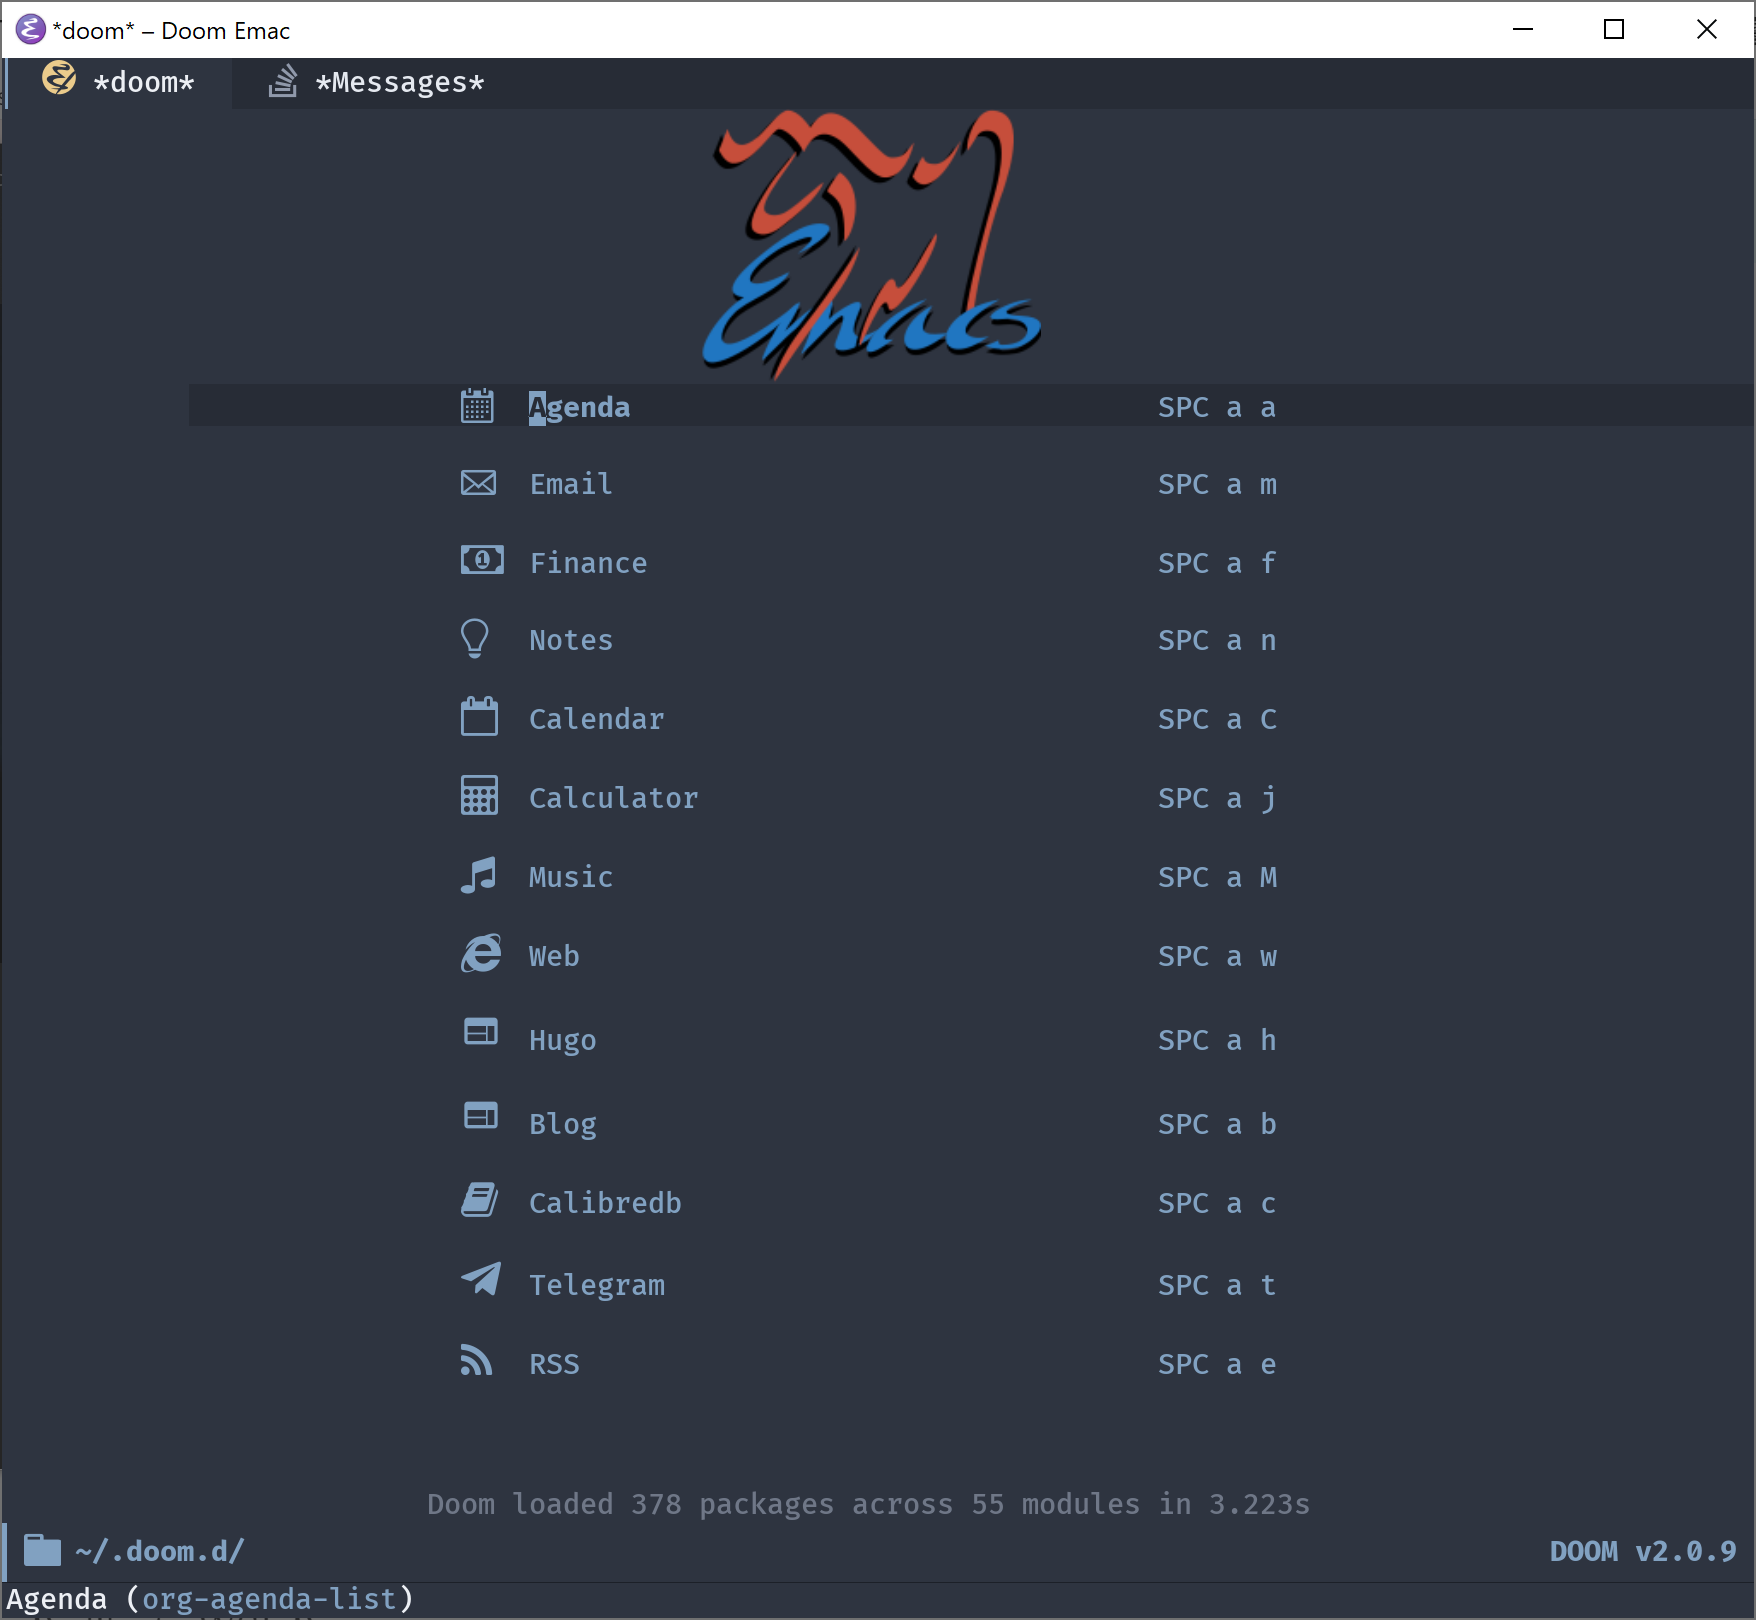
\includegraphics[width=.9\linewidth]{emacs.png}
\end{center}

Do you think Emacs's performance in windows is bad? Do you really want to use a native Speed Emacs in Windows? Do you hate the unnatural path transition between windows convention and Linux convention? Do you feel frustrated when you try to install and configure Emacs in WSL? Do you just want to taste the power of Emacs running in WSL 2?

This tutorial may help you :)

\section{What is WSL?}
\label{sec:org59faa84}
Earlier on August 2, 2016, Microsoft released \textbf{Windows Subsystem for Linux} (WSL), enabling the native way to run Linux Tools in Windows 10 and Windows Server 2019.

In May 2019, WSL 2 was introduced, by importing the Real Linux Kernel through Hyper-V features (in a Virtual Machine Environment), providing the users with the full \& immerse way to work with Linux under windows, with 20 times the read/write performances of WSL 1.

For Windows Emacs Users, here are some advantages/disadvantages for you to consider before switching the WSL 2:

\subsection{Advantages}
\label{sec:orgb43f397}
\begin{enumerate}
\item The performance of \href{https://github.com/magit/magit}{Magit} is way faster than the GNU compiled original windows \href{https://ftp.gnu.org/gnu/emacs/windows/emacs-27/}{Emacs-27} binaries.
\item The Font Rendering is better.
\item No flickering.
\item \href{https://docs.microsoft.com/en-us/windows/wsl/interop}{interoperability} between Windows and Linux.
\item Native OneDrive support.
\item Super fast boot up time for Emacs.
\end{enumerate}

\subsection{Disadvantages}
\label{sec:org5bae775}
\begin{enumerate}
\item The network configuration is a pain, workaround is available.
\item X11 may lost connection when network changes.
\end{enumerate}

\subsection{More Details}
\label{sec:orgce6ffa0}
More details of the differences between WSL 1 and WSL 2, check \url{https://docs.microsoft.com/en-us/windows/wsl/compare-versions}.


\section{Taste WSL 2}
\label{sec:orgfbaaffc}
\subsection{Install and enable WSL 2}
\label{sec:org21b82b0}
\subsubsection{Update Windows 10}
\label{sec:org62593cc}
The first step is to make sure you have updated to the latest Windows 10. For Windows 10 Versions 1903 \& 1909 users, make sure the minor version number is \textbf{1049}, according to Microsoft's \href{https://devblogs.microsoft.com/commandline/wsl-2-support-is-coming-to-windows-10-versions-1903-and-1909/}{Devblog}.

\subsubsection{Install WSL 2}
\label{sec:org486b32f}
\begin{verbatim}
Enable-WindowsOptionalFeature -Online -FeatureName Microsoft-Windows-Subsystem-Linux
\end{verbatim}

\subsubsection{Enable WSL 2}
\label{sec:org393eafd}
\begin{verbatim}
dism.exe /online /enable-feature /featurename:VirtualMachinePlatform /all /norestart
\end{verbatim}

\subsubsection{Check WSL version}
\label{sec:org8c494f1}
\begin{verbatim}
wsl -l -v
\end{verbatim}
There are many people who may be not able to run the above commands, just make sure you have updated to the latest windows.
\url{https://devblogs.microsoft.com/commandline/wsl-2-support-is-coming-to-windows-10-versions-1903-and-1909/}

\subsubsection{Set default WSL version to 2}
\label{sec:org54fe6e3}
\begin{verbatim}
wsl.exe --set-default-version 2
\end{verbatim}
All later WSL Distros are installed will be WSL 2. No worries, you can switch between WSL 1 and WSL 2 with just one command without pain, just do it\textasciitilde{}

\subsubsection{Install Ubuntu 18.04 in Microsoft Store}
\label{sec:org38dd771}
\begin{center}
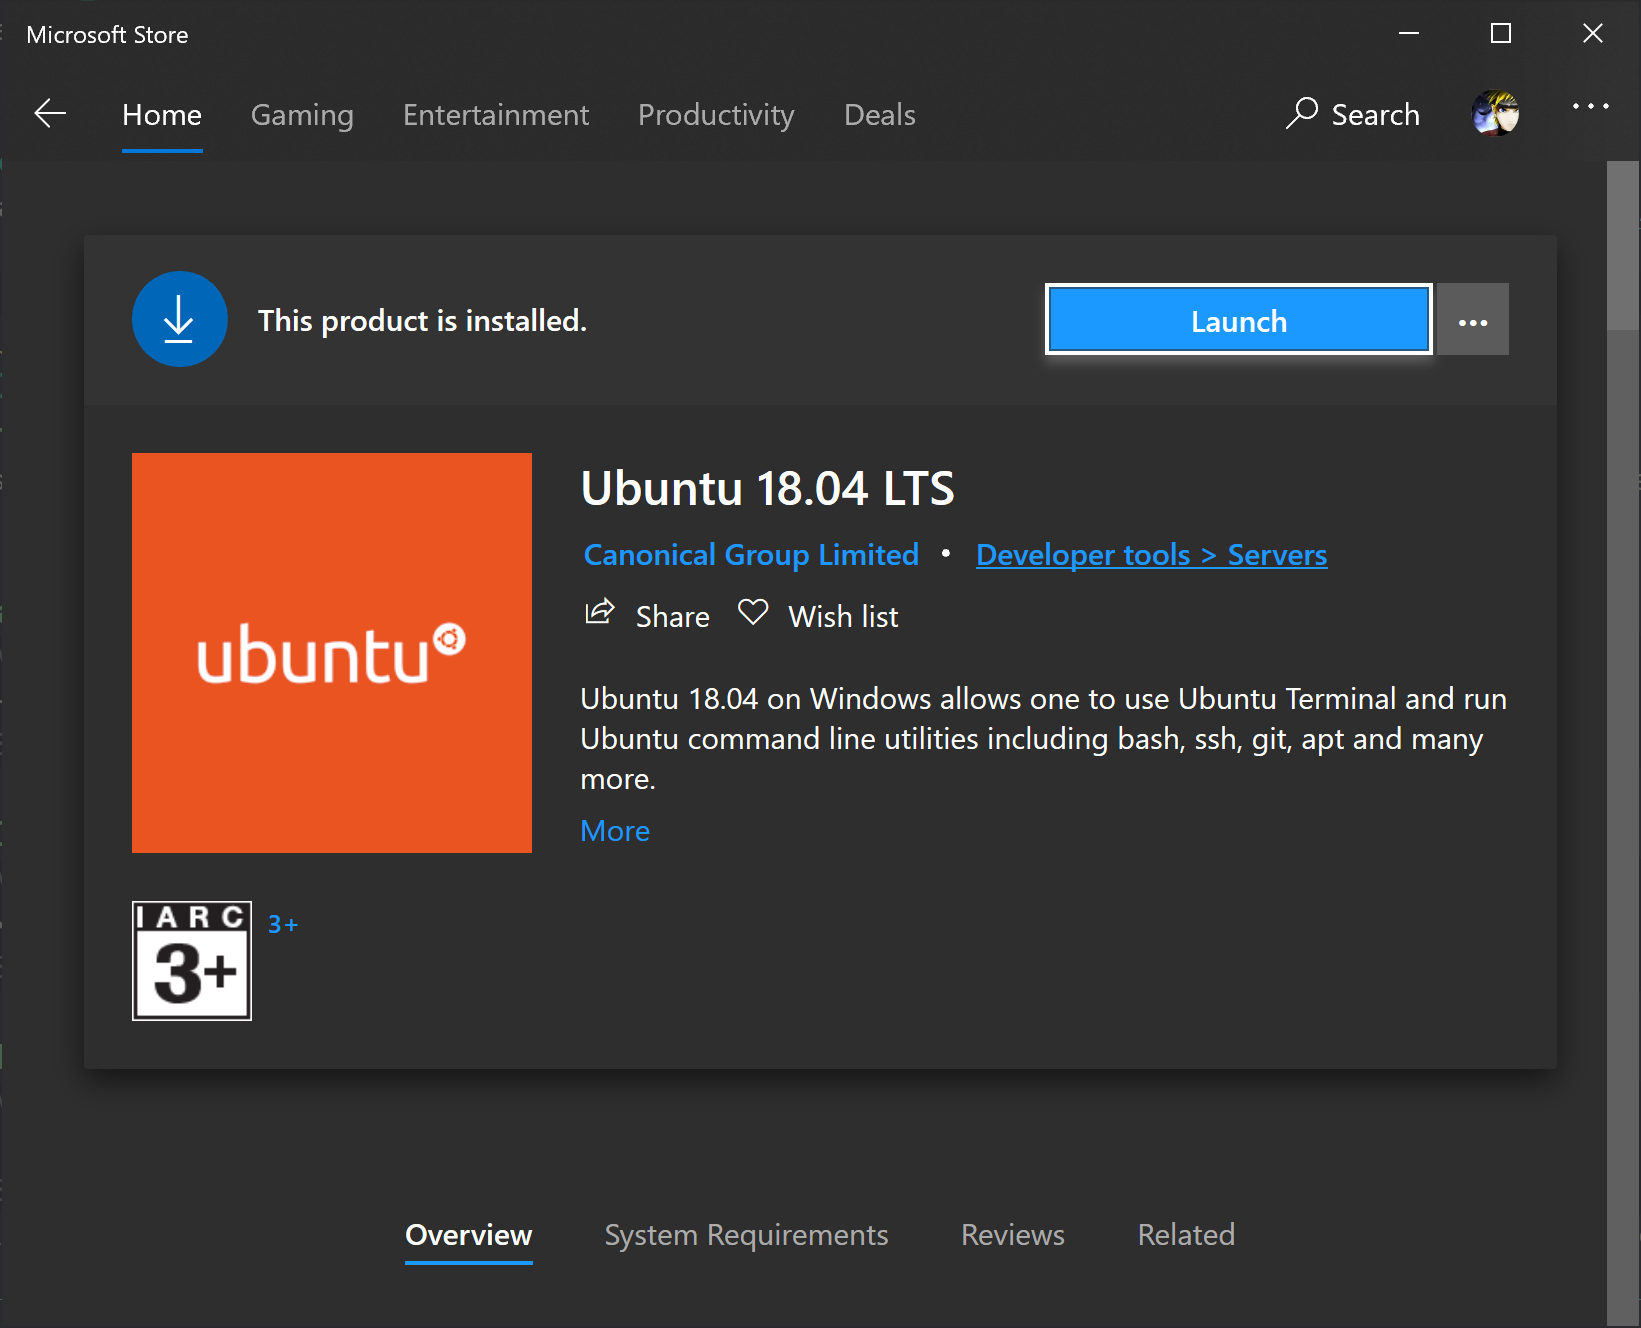
\includegraphics[width=.9\linewidth]{ubuntu18.04.png}
\end{center}

\subsubsection{Optional: Convert WSL 1 to WSL 2}
\label{sec:orgd98dfa1}
If you already installed some Distros before but they are in WSL 1, no worries, it is very easy to switch from WSL 1 to WSL 2:
\begin{verbatim}
wsl.exe --set-version Ubuntu-18.04 2
\end{verbatim}

\subsection{Choosing the terminal}
\label{sec:orgcf124de}
The first step to talk to WSL 2 is via Terminal Applications. In macOS, we have \href{https://iterm2.com/}{iTerm2}, how about Windows? You may wonder we could just use the default Ubuntu Terminal, but it lacks UTF8 and Unicode supports, and only a few configuration options. Apparently, it is not the best option. We just need a more powerful and modern terminal. Luckily, Microsoft brings us another great product - \href{https://github.com/microsoft/terminal}{Windows Terminal}, and it is ranked with \textbf{67.6k} stars in GitHub up to the time this article composed.

Windows Terminal has the following benefits compared with other terminals:
\begin{enumerate}
\item Windows Terminal is multi-tabs and multi-panels.
\item UTF8 \& Unicode support.
\item Supports Command Prompt, PowerShell, and WSL.
\item GPU accelerated Text Rendering Engine.
\item Custom Themes, styles and configurations.
\item Modern and user-friendly.
\item Open Source and Official Support.
\end{enumerate}

\subsubsection{Install windows Terminal in Microsoft Store}
\label{sec:org2ac4899}
\begin{center}
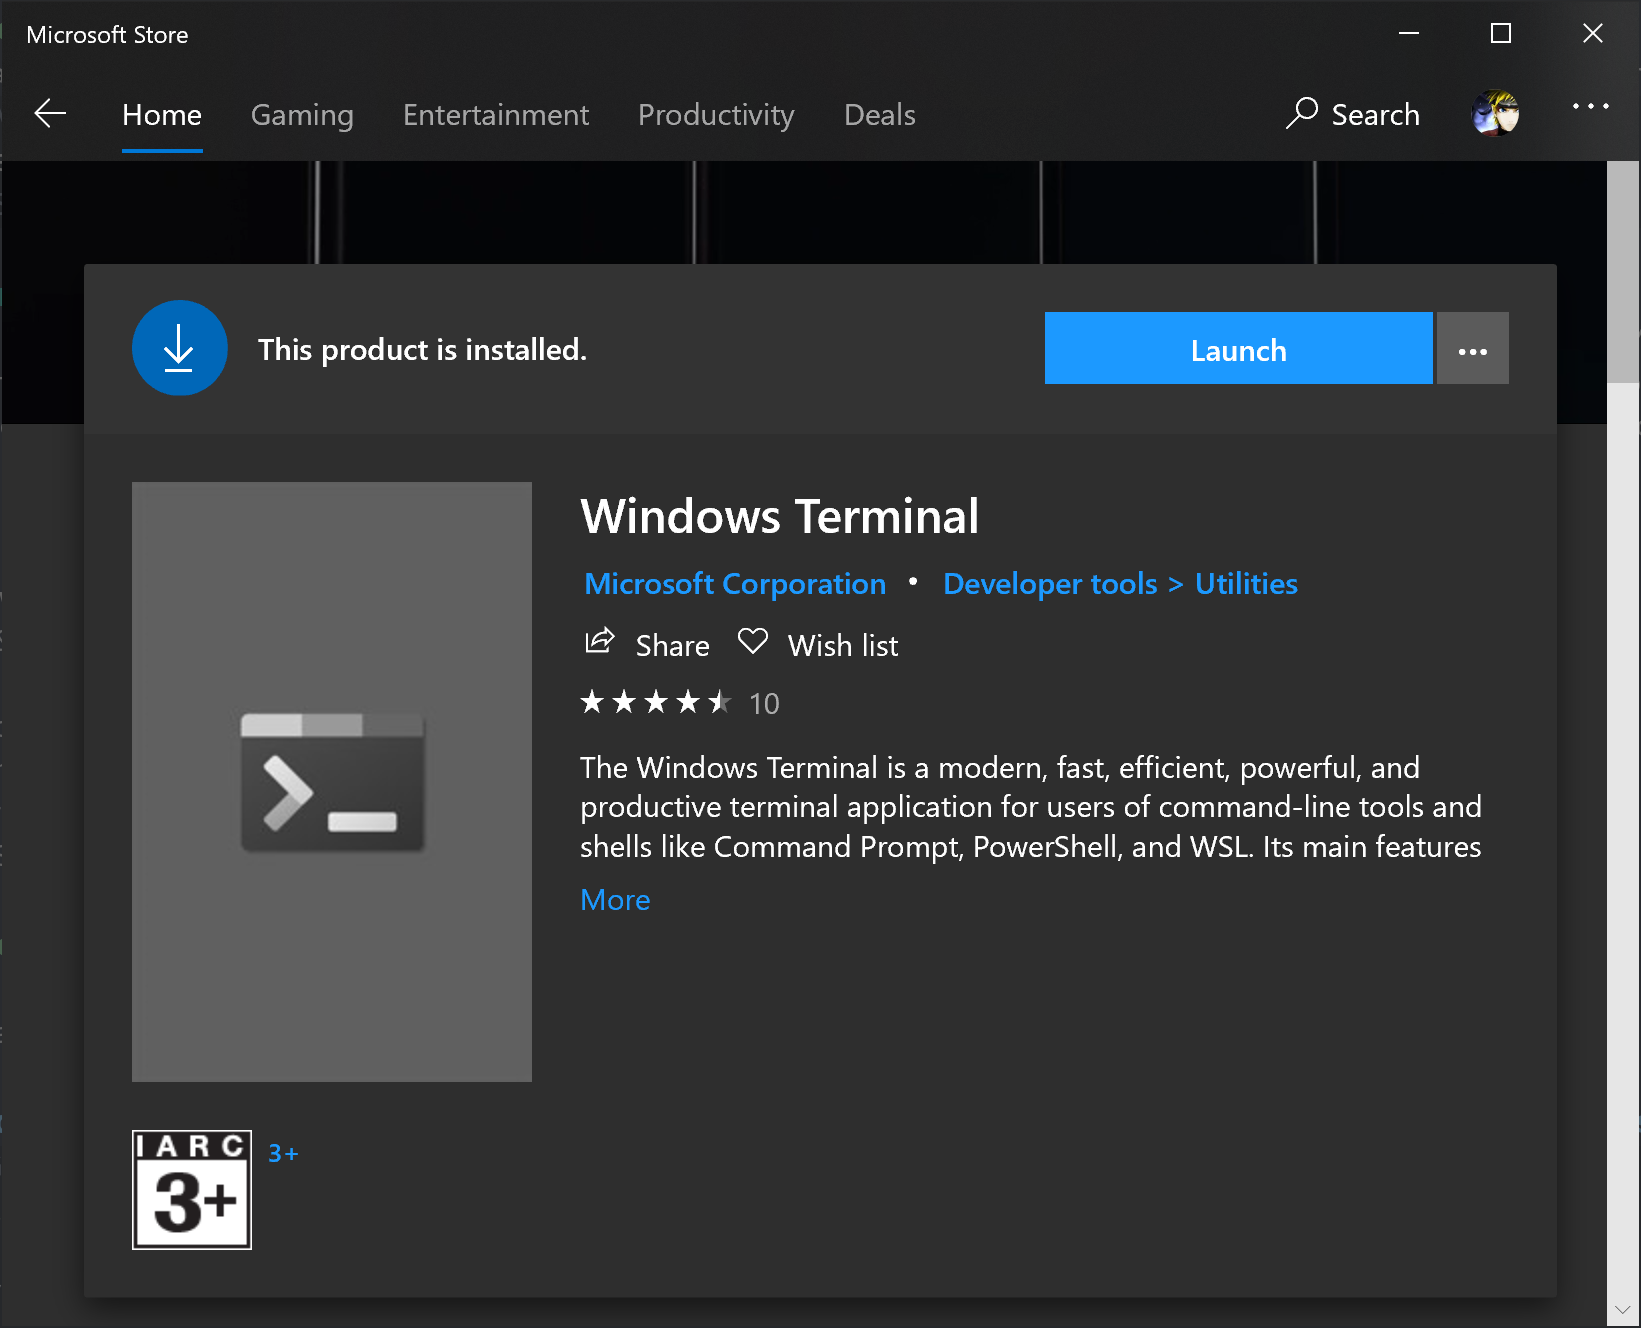
\includegraphics[width=.9\linewidth]{windows-terminal.png}
\end{center}

\subsubsection{Windows Terminal}
\label{sec:org197d2c1}
Windows Terminal's setting is implemented in a json file - \texttt{settings.json}, every time you modify and save the file, it will take effects immediately, nice!

\begin{enumerate}
\item Add ``cursorShape'' and ``fontFace'' to the ``defaults'' section, it will apply on all tabs
\label{sec:org539e60d}
\begin{verbatim}
"defaults":
{
    // Put settings here that you want to apply to all profiles.
    "cursorShape": "filledBox" ,
    "fontFace": "JetBrains Mono"
}
\end{verbatim}

\item Update the home directory
\label{sec:org74b6908}
\begin{verbatim}
{
    "guid": "{c6eaf9f4-32a7-5fdc-b5cf-066e8a4b1e40}",
    "hidden": false,
    "name": "Ubuntu-18.04",
    "source": "Windows.Terminal.Wsl",
    "startingDirectory": "//wsl$/Ubuntu-18.04/home/damonchan"

}
\end{verbatim}

\item Disable keyboard cursor blink
\label{sec:org43fdb20}
Disable globally in keyboard setting:
\begin{center}
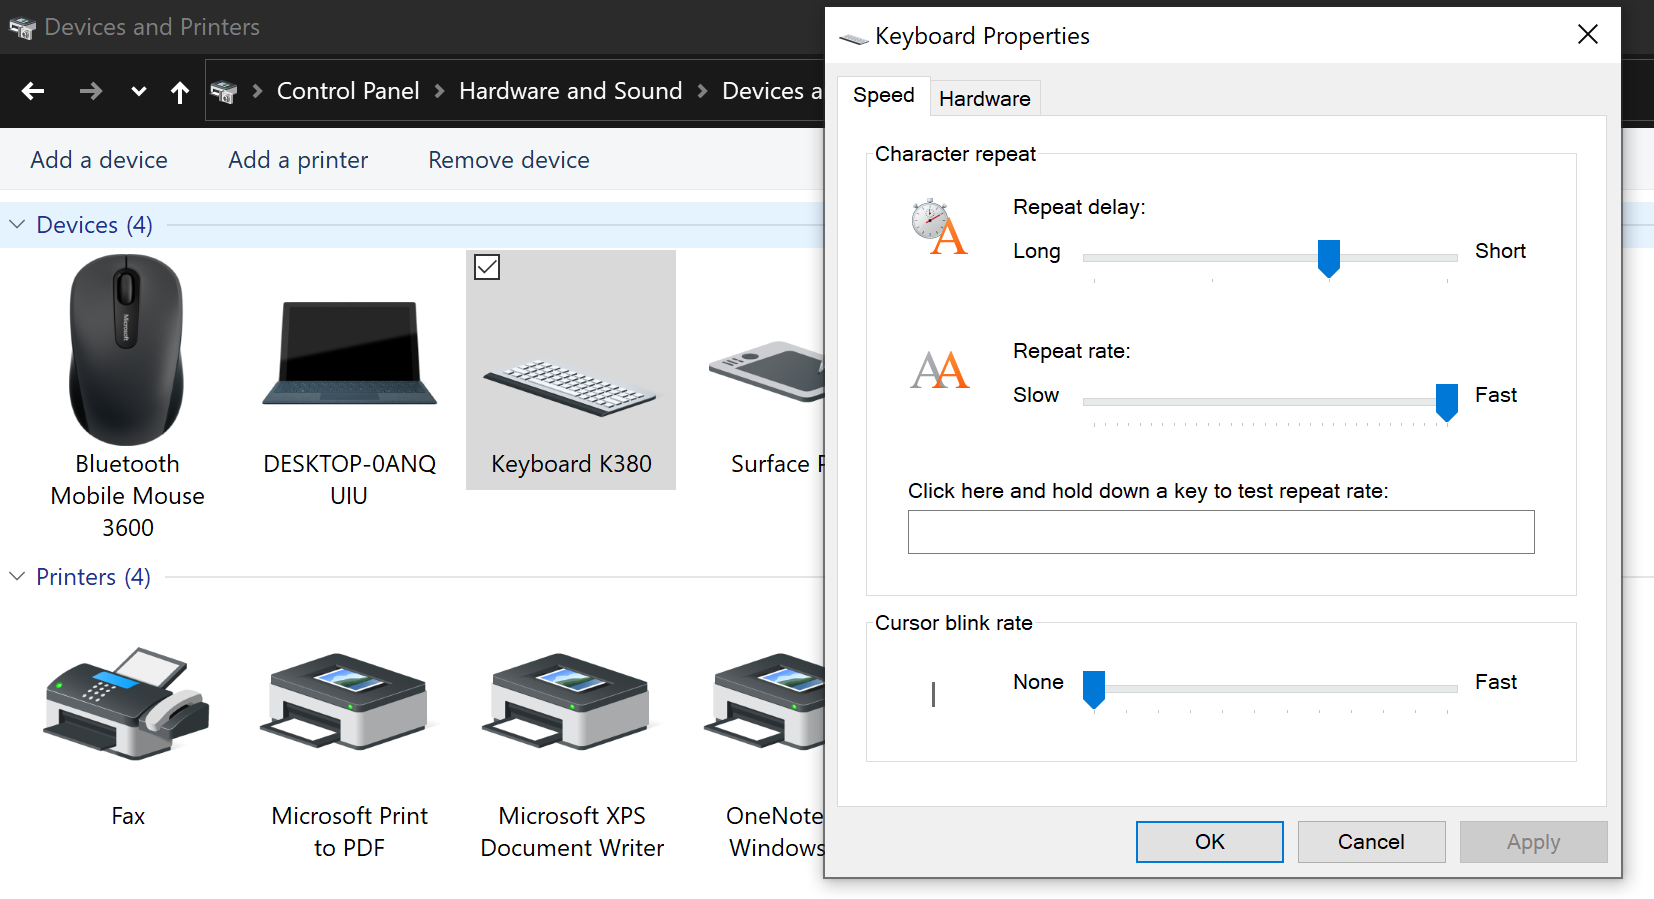
\includegraphics[width=.9\linewidth]{UnblinkCursor.png}
\end{center}
\end{enumerate}

\subsection{zsh}
\label{sec:org2d0ce78}
I like to use zsh which provides more enhancement and configuration options compared with Bash.
\begin{verbatim}
sudo apt install zsh
chsh -s $(which zsh)
sh -c "$(curl -fsSL https://raw.githubusercontent.com/robbyrussell/oh-my-zsh/master/tools/install.sh)"
\end{verbatim}

\subsection{Fonts}
\label{sec:org0bfb6e0}
Just create a soft link from Windows to Ubuntu:
\begin{verbatim}
ln -s /mnt/c/Windows/Fonts ~/.fonts
fc-cache -fv
\end{verbatim}

\subsection{OneDrive}
\label{sec:org02d82f9}
Just link Windows OneDrive Root Directory to Ubuntu:
\begin{verbatim}
ln -s /mnt/c/Users/elecm/OneDrive ~/OneDrive
\end{verbatim}

\subsection{X11 Server (VcXsrv)}
\label{sec:org962fdbf}
In this tutorial, we choose VcXsrv as X11 server.

\subsubsection{Install VcXsrv}
\label{sec:org9bb69ed}
\begin{verbatim}
choco install vcxsrv
\end{verbatim}

\subsubsection{Configure VcXsrv}
\label{sec:org1f3684b}
\begin{enumerate}
\item Start XLunch (VcXsrv)
\begin{itemize}
\item Multiple windows -> Display number: -1 -> Next
\begin{center}
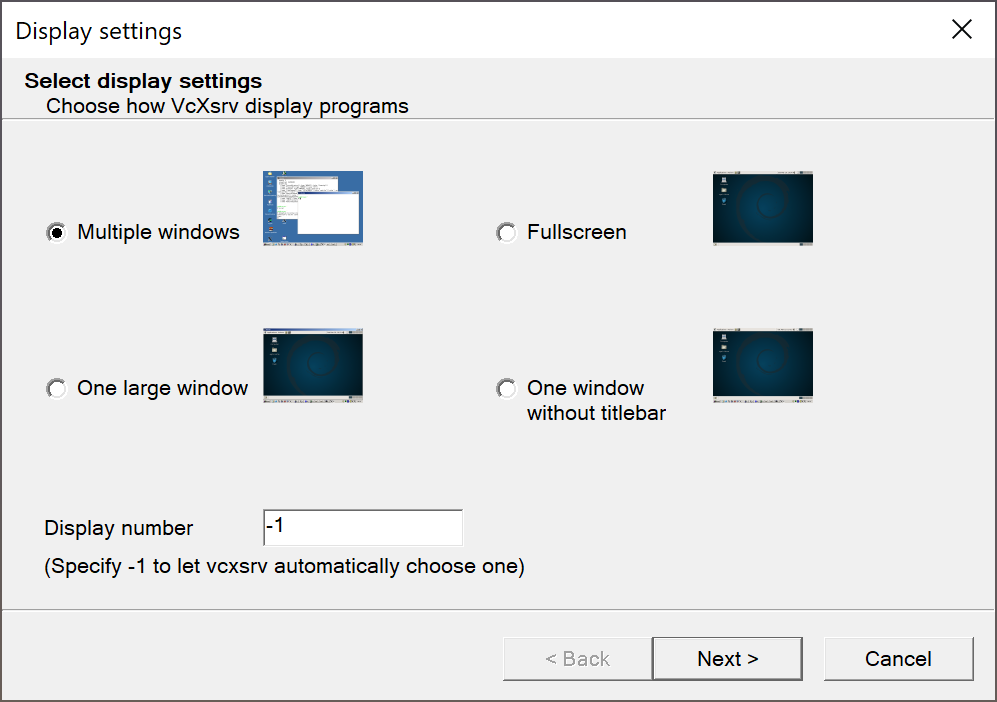
\includegraphics[width=.9\linewidth]{vcxsrv-1.png}
\end{center}
\item Start no client
\begin{center}
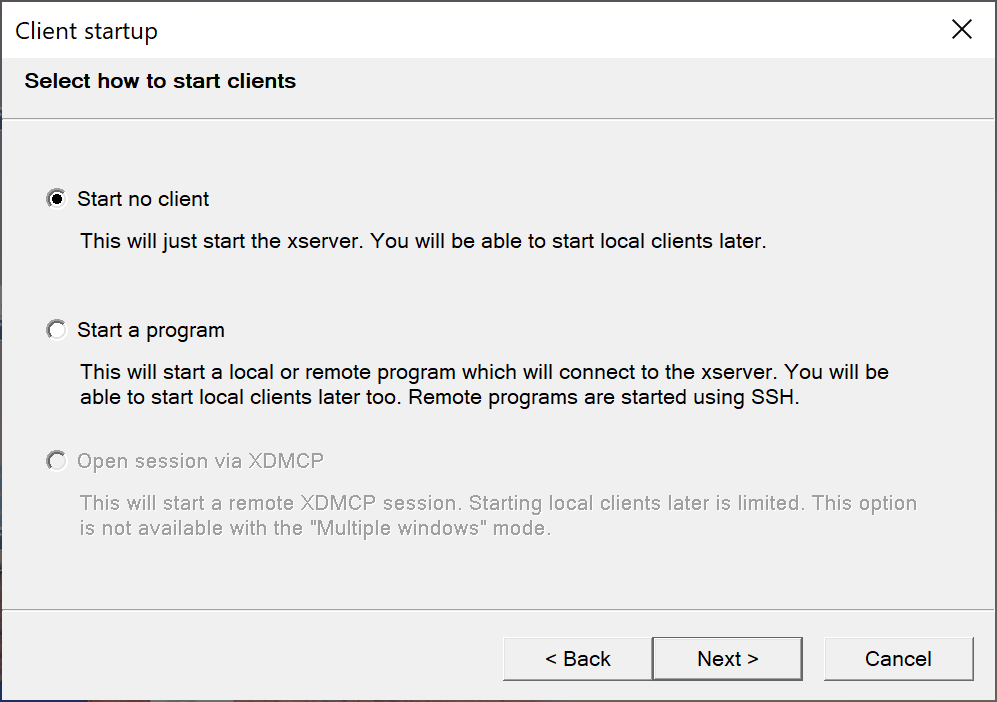
\includegraphics[width=.9\linewidth]{vcxsrv-2.png}
\end{center}
\item Tick Clipboard, Primary Selection, Native opengl, Disable access control (If you use \texttt{socat} to do X11 forwarding, Access control can be enabled, check \ref{sec:orgd4d334b} below) -> Next
\begin{center}
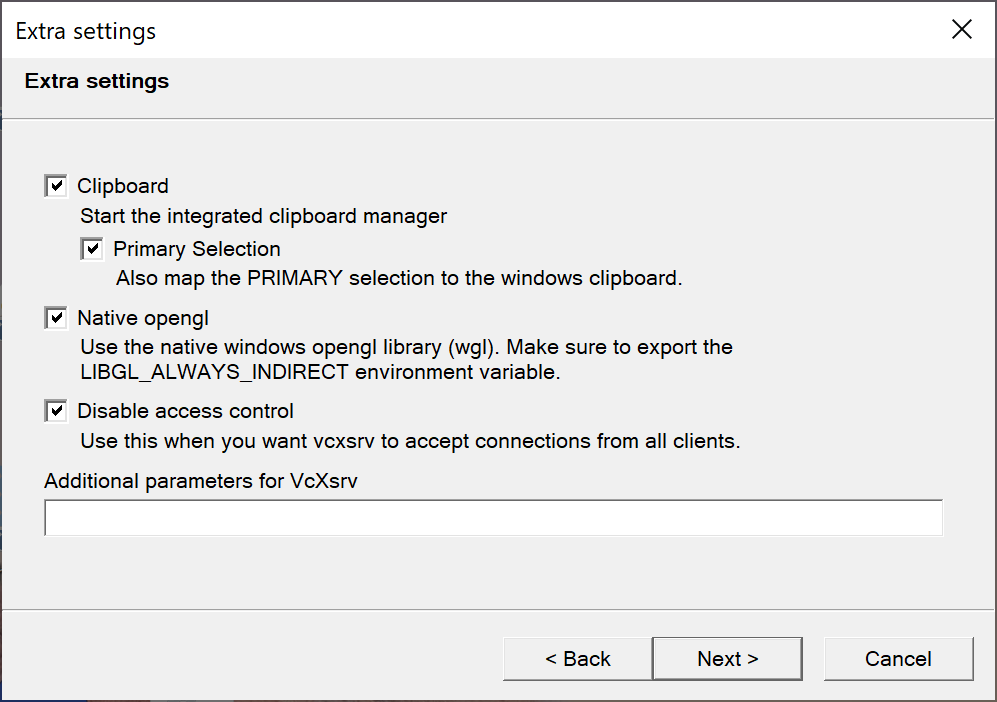
\includegraphics[width=.9\linewidth]{vcxsrv-3.png}
\end{center}
\item Save configuration
PS:
\begin{itemize}
\item Press ``Win + R'' -> insert \texttt{shell:startup} -> Press Enter
\item Save to startup can start X11 server when system boots
\end{itemize}
\item Finish
\end{itemize}
\item allow both Private and Public network in windows firewall setting
\texttt{Control Panel\textbackslash{}System and Security\textbackslash{}Windows Defender Firewall\textbackslash{}Allowed apps}
\begin{center}
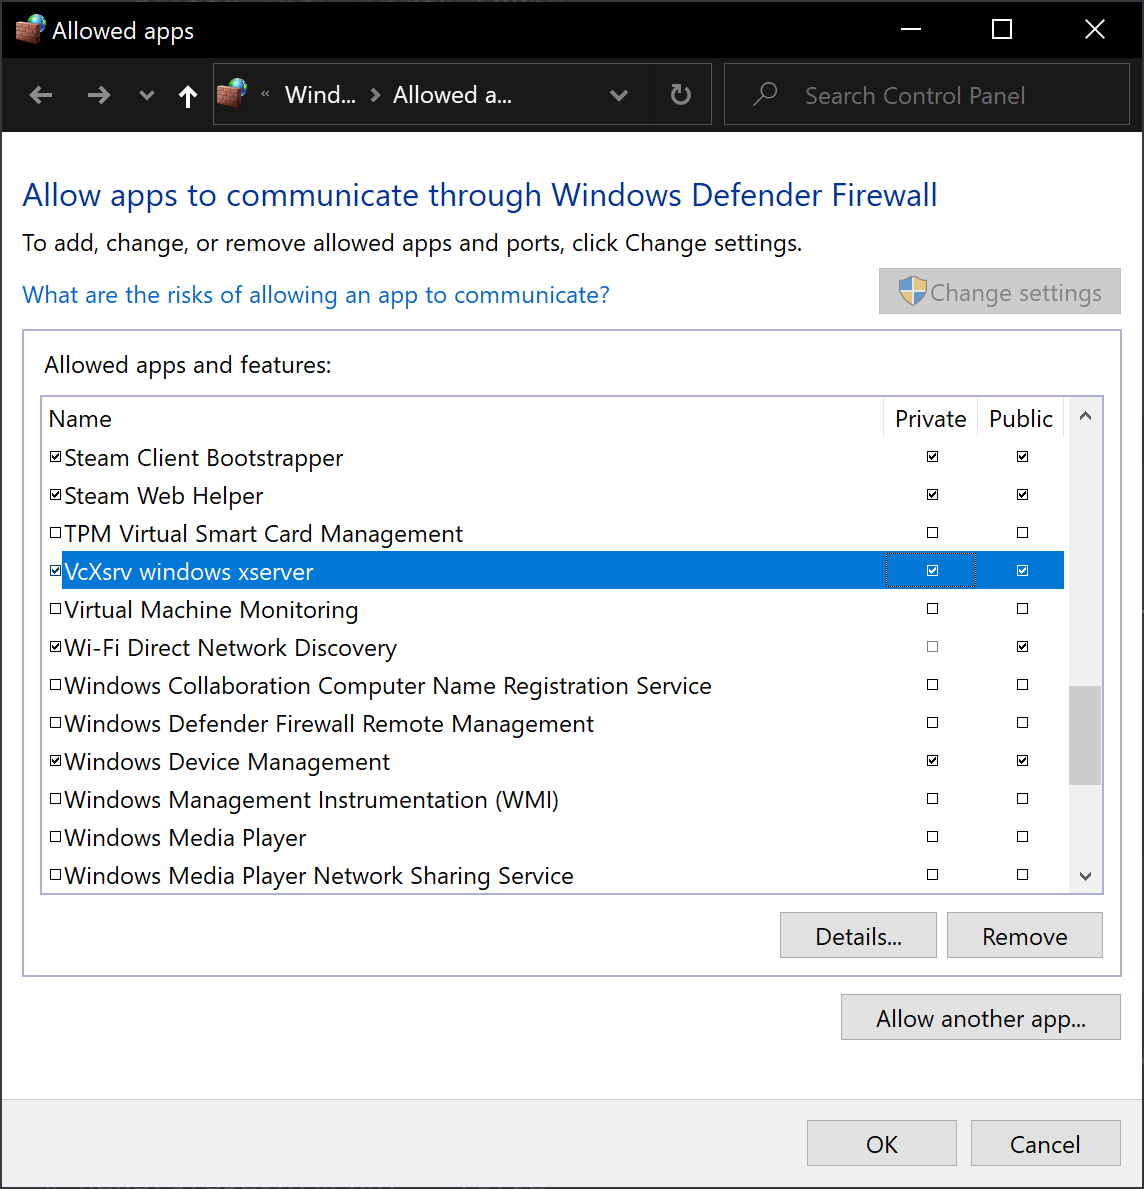
\includegraphics[width=.9\linewidth]{vcxsrv-5.png}
\end{center}
\end{enumerate}

\subsubsection{Disable \texttt{/etc/resolv.conf} generation}
\label{sec:org4d8090e}
We disable \texttt{/etc/resolv.conf} generation, so that we can use custom name servers which points to google.
\texttt{vi /etc/wsl.conf}
\begin{verbatim}
[network]
generateResolvConf = false
\end{verbatim}

\subsubsection{Setup custom name servers and point to google}
\label{sec:org9002267}
\texttt{vi /etc/resolv.conf}
\begin{verbatim}
# This file was automatically generated by WSL. To stop automatic generation of this file, add the following entry to /etc/wsl.conf:
# [network]
# generateResolvConf = false
nameserver 8.8.8.8
nameserver 8.8.4.4
\end{verbatim}

\subsubsection{Export DISPLAY and LIBGL\textsubscript{ALWAYS}\textsubscript{INDIRECT} settings to \texttt{\textasciitilde{}/.zshrc}}
\label{sec:org01a75c0}
\texttt{vi \textasciitilde{}/.zshrc}
\begin{verbatim}
export DISPLAY=$(ip route | awk '{print $3; exit}'):0
export LIBGL_ALWAYS_INDIRECT=1
\end{verbatim}

\subsubsection{Other Methods}
\label{sec:orgd4d334b}
There is another way to enable the X11 forwarding through \href{https://github.com/microsoft/WSL/issues/4619\#issuecomment-678652118}{socat}, check \href{https://github.com/microsoft/WSL/issues/4619\#issuecomment-678652118}{this github issue.} It is more safe but has some performance lost.

\subsubsection{HiDPI}
\label{sec:orgf395e73}
\begin{enumerate}
\item Right click \texttt{XLaunch} (VcXsrv) -> Compatibility -> Change high DPI settings -> Tick Override high DPI scaling Behavior, Application.
\begin{center}
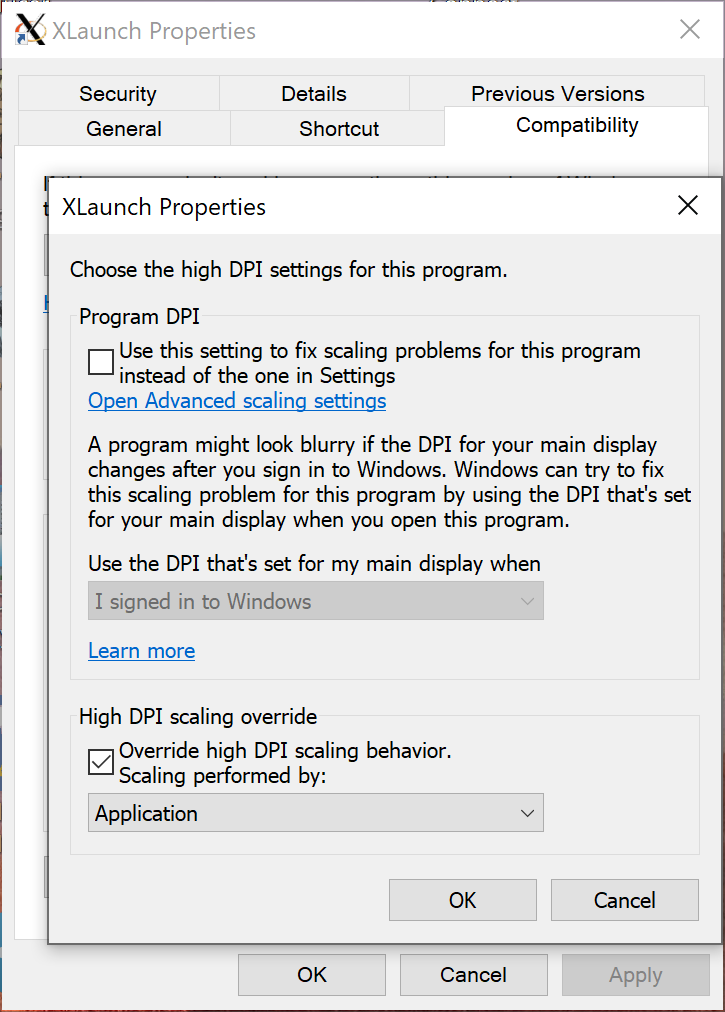
\includegraphics[width=.9\linewidth]{vcxsrv-4.png}
\end{center}
\item Add the following statement to \texttt{.zshrc}
\end{enumerate}
\begin{verbatim}
export GDK_SCALE=2
\end{verbatim}

\subsubsection{Bigger Cursor}
\label{sec:org315c6fc}

Supposed VcXsrv is installed in \texttt{C:\textbackslash{}Program Files\textbackslash{}VcXsrv\textbackslash{}},

\begin{enumerate}
\item Install big-cursor
\begin{verbatim}
    sudo apt install big-cursor
\end{verbatim}
\item Rename
\texttt{C:\textbackslash{}Program Files\textbackslash{}VcXsrv\textbackslash{}fonts\textbackslash{}misc\textbackslash{}cursor.pcf.gz} to \texttt{C:\textbackslash{}Program Files\textbackslash{}VcXsrv\textbackslash{}fonts\textbackslash{}misc\textbackslash{}cursor-small.pcf.gz}
\item Copy \texttt{/usr/share/fonts/X11/misc/big-cursor.pcf.gz} from WSL to as \texttt{C:\textbackslash{}Program Files\textbackslash{}VcXsrv\textbackslash{}fonts\textbackslash{}misc\textbackslash{}cursor.pcf.gz}
\end{enumerate}

\subsection{Setup Emacs}
\label{sec:org5d2392f}
Let's dive into the meat of Compiling and installing the latest \textbf{Emacs 27.1}!
\subsubsection{install dependencies}
\label{sec:org0723e69}
\begin{verbatim}
sudo apt install -y autoconf automake autotools-dev bsd-mailx build-essential \
    diffstat gnutls-dev imagemagick libasound2-dev libc6-dev libdatrie-dev \
    libdbus-1-dev libgconf2-dev libgif-dev libgnutls28-dev libgpm-dev libgtk2.0-dev \
    libgtk-3-dev libice-dev libjpeg-dev liblockfile-dev liblqr-1-0 libm17n-dev \
    libmagickwand-dev libncurses5-dev libncurses-dev libotf-dev libpng-dev \
    librsvg2-dev libsm-dev libthai-dev libtiff5-dev libtiff-dev libtinfo-dev libtool \
    libx11-dev libxext-dev libxi-dev libxml2-dev libxmu-dev libxmuu-dev libxpm-dev \
    libxrandr-dev libxt-dev libxtst-dev libxv-dev quilt sharutils texinfo xaw3dg \
    xaw3dg-dev xorg-dev xutils-dev zlib1g-dev libjansson-dev libxaw7-dev \
    libselinux1-dev libmagick++-dev libacl1-dev gir1.2-javascriptcoregtk-4.0 \
    gir1.2-webkit2-4.0 libenchant1c2a libglvnd-core-dev libicu-le-hb-dev \
    libidn2-0-dev libjavascriptcoregtk-4.0-dev liboss4-salsa2 libsoup2.4-dev \
    libsystemd-dev libwebkit2gtk-4.0-dev libx11-xcb-dev libxcb-dri2-0-dev \
    libxcb-dri3-dev libxcb-glx0-dev libxcb-present-dev libxshmfence-dev \
    x11proto-composite-dev x11proto-core-dev x11proto-damage-dev \
    x11proto-fixes-dev
\end{verbatim}

\subsubsection{Download, compile and install}
\label{sec:org9c15865}
\begin{verbatim}
cd ~
wget https://ftp.gnu.org/pub/gnu/emacs/emacs-27.1.tar.gz
tar -xzvf emacs-27.1.tar.gz
cd emacs-27.1
./configure
make
sudo make install
rm ~/emacs-27.1.tar.gz
\end{verbatim}

\subsubsection{Install doom}
\label{sec:org6e10c66}
\begin{verbatim}
git clone --depth 1 https://github.com/hlissner/doom-emacs ~/.emacs.d
~/.emacs.d/bin/doom install
\end{verbatim}

\subsubsection{Start Emacs}
\label{sec:org638f6c8}
\begin{verbatim}
emacs
\end{verbatim}

Please notice:
\begin{enumerate}
\item The first time to start Emacs may need some times (Every time the first time to start Emacs after system boots, it also needs some time at times), font setting, x11 checking, sound checking etc, please wait a moment. Normally it will finish within one or two minute.
\item After refreshing font setting through \texttt{fc-cache -fv}, Emacs will take some time to configure the font setting, but it will only conduct one time.
\item The second time to start Emacs will resume to the normal startup time.
\end{enumerate}

\subsection{Fix WSL\textsubscript{INTEROP} issue}
\label{sec:org5a60202}
When you start Emacs, it will create another \texttt{interop} file, it make us can not start windows programs in Emacs, we can make it to use the one same \texttt{interop} file with the terminal.

Add the following to \texttt{.zshrc}
\begin{verbatim}
# fix interop
fix_wsl2_interop() {
	for i in $(pstree -np -s $$ | grep -o -E '[0-9]+'); do
		if [[ -e "/run/WSL/${i}_interop" ]]; then
			export WSL_INTEROP=/run/WSL/${i}_interop
		fi
	done
}

~/.emacs.d/bin/doom env > /dev/null 2>&1
\end{verbatim}

\subsection{Optional: Setup Python Development Environment}
\label{sec:orgd144a3d}
\subsubsection{pyenv}
\label{sec:org9afd117}
\begin{verbatim}
sudo apt-get install git gcc make openssl libssl-dev libbz2-dev libreadline-dev libsqlite3-dev libffi-dev
git clone https://github.com/pyenv/pyenv.git ~/.pyenv
echo 'export PYENV_ROOT="$HOME/.pyenv"' >> ~/.zshrc
echo 'export PATH="$PYENV_ROOT/bin:$PATH"' >> ~/.zshrc
echo -e 'if command -v pyenv 1>/dev/null 2>&1; then\n  eval "$(pyenv init -)"\nfi' >> ~/.zshrc
pyenv install 3.7.9
pyenv global 3.7.9
\end{verbatim}

\subsubsection{mypyls}
\label{sec:org21a60b5}
\textbf{mspyls} can be installed by typing \texttt{M-x lsp-install-server RET mspyls}.

\subsection{Optional: Setup Node.js Development Environment}
\label{sec:org5f5c095}
\subsubsection{node}
\label{sec:orgdc34941}
Install nvm
\begin{verbatim}
curl -o- https://raw.githubusercontent.com/nvm-sh/nvm/v0.35.3/install.sh | bash
\end{verbatim}

Add to .zshrc
\begin{verbatim}
export NVM_DIR="$HOME/.nvm"
[ -s "$NVM_DIR/nvm.sh" ] && \. "$NVM_DIR/nvm.sh"  # This loads nvm
[ -s "$NVM_DIR/bash_completion" ] && \. "$NVM_DIR/bash_completion"  # This loads nvm bash_completion
\end{verbatim}

\begin{verbatim}
nvm install --lts
nvm use --lts
npm i -g javascript-typescript-langserver
.emacs.d/bin/doom sync
\end{verbatim}


\subsection{Optional: Setup Rust Development Environment}
\label{sec:org07cf3fe}
\begin{verbatim}
curl --proto '=https' --tlsv1.2 -sSf https://sh.rustup.rs | sh
rustup component add rust-src
sudo curl -L https://github.com/rust-analyzer/rust-analyzer/releases/latest/download/rust-analyzer-linux -o /usr/bin/rust-analyzer
sudo chmod +x /usr/bin/rust-analyzer
cargo install cargo-check
rustup component add clippy-preview
\end{verbatim}


\subsection{Optional: Install other useful packages}
\label{sec:orgf77da72}
\subsubsection{apt}
\label{sec:org8d706df}
With \texttt{apt}
\begin{verbatim}
sudo apt install calibre sqlite3 pandoc
\end{verbatim}

\subsubsection{pdf-tools}
\label{sec:org21c238d}
\begin{verbatim}
sudo apt install libpng-dev zlib1g-dev libpoppler-glib-dev libpoppler-private-dev
M-x pdf-tools-install
\end{verbatim}

\subsubsection{rga}
\label{sec:org1445cfd}
\begin{verbatim}
sudo apt install build-essential pandoc poppler-utils ffmpeg
wget https://github.com/phiresky/ripgrep-all/releases/download/v0.9.6/ripgrep_all-v0.9.6-x86_64-unknown-linux-musl.tar.gz
tar -zxvf ripgrep_all-v0.9.6-x86_64-unknown-linux-musl.tar.gz
cd ripgrep_all-v0.9.6-x86_64-unknown-linux-musl
sudo cp rga /usr/bin
sudo cp rga-preproc /usr/bin
\end{verbatim}

\subsubsection{Rime}
\label{sec:org2a9face}
\begin{enumerate}
\item Install and setup Rime
\label{sec:orgb66578a}
\begin{verbatim}
sudo apt install git build-essential cmake libboost-all-dev libgoogle-glog-dev libleveldb-dev libmarisa-dev libopencc-dev libyaml-cpp-dev libgtest-dev
cd /usr/src/gtest
sudo cmake CMakeLists.txt
sudo make
#copy or symlink libgtest.a and libgtest_main.a to your /usr/lib folder
sudo cp *.a /usr/lib
cd ~/.emacs.d/librime
make
sudo make install
sudo apt-get install ibus-rime
\end{verbatim}

PS: It is better to not share Rime User folder between windows and WSL, it may cause troubles.

In Emacs
\begin{verbatim}
M-x rime-compile-module
\end{verbatim}

\item plum
\label{sec:org7d743d4}
\begin{verbatim}
curl -fsSL https://git.io/rime-install | bash
# rime_dir="$HOME/.rime" bash rime-install
\end{verbatim}
\end{enumerate}

\subsubsection{sdcv}
\label{sec:orgb32eb9c}
\begin{verbatim}
sudo apt install stardict sdcv
\end{verbatim}

\subsubsection{telega}
\label{sec:orgb680c09}
\begin{verbatim}
sudo apt install gperf
git clone https://github.com/tdlib/td.git
cd td
mkdir build && cd build && cmake ../
make
sudo make install
git clone https://github.com/zevlg/telega.el
cd telega.el
make && make install
\end{verbatim}


\subsection{An .zshrc example}
\label{sec:orgcbb2cc1}

\begin{verbatim}
# If you come from bash you might have to change your $PATH.
# export PATH=$HOME/bin:/usr/local/bin:$PATH

# Path to your oh-my-zsh installation.
export ZSH="/home/damonchan/.oh-my-zsh"

# Set name of the theme to load --- if set to "random", it will
# load a random theme each time oh-my-zsh is loaded, in which case,
# to know which specific one was loaded, run: echo $RANDOM_THEME
# See https://github.com/ohmyzsh/ohmyzsh/wiki/Themes
ZSH_THEME="robbyrussell"

# Set list of themes to pick from when loading at random
# Setting this variable when ZSH_THEME=random will cause zsh to load
# a theme from this variable instead of looking in $ZSH/themes/
# If set to an empty array, this variable will have no effect.
# ZSH_THEME_RANDOM_CANDIDATES=( "robbyrussell" "agnoster" )

# Uncomment the following line to use case-sensitive completion.
# CASE_SENSITIVE="true"

# Uncomment the following line to use hyphen-insensitive completion.
# Case-sensitive completion must be off. _ and - will be interchangeable.
# HYPHEN_INSENSITIVE="true"

# Uncomment the following line to disable bi-weekly auto-update checks.
# DISABLE_AUTO_UPDATE="true"

# Uncomment the following line to automatically update without prompting.
# DISABLE_UPDATE_PROMPT="true"

# Uncomment the following line to change how often to auto-update (in days).
# export UPDATE_ZSH_DAYS=13

# Uncomment the following line if pasting URLs and other text is messed up.
# DISABLE_MAGIC_FUNCTIONS="true"

# Uncomment the following line to disable colors in ls.
# DISABLE_LS_COLORS="true"

# Uncomment the following line to disable auto-setting terminal title.
# DISABLE_AUTO_TITLE="true"

# Uncomment the following line to enable command auto-correction.
# ENABLE_CORRECTION="true"

# Uncomment the following line to display red dots whilst waiting for completion.
# COMPLETION_WAITING_DOTS="true"

# Uncomment the following line if you want to disable marking untracked files
# under VCS as dirty. This makes repository status check for large repositories
# much, much faster.
# DISABLE_UNTRACKED_FILES_DIRTY="true"

# Uncomment the following line if you want to change the command execution time
# stamp shown in the history command output.
# You can set one of the optional three formats:
# "mm/dd/yyyy"|"dd.mm.yyyy"|"yyyy-mm-dd"
# or set a custom format using the strftime function format specifications,
# see 'man strftime' for details.
# HIST_STAMPS="mm/dd/yyyy"

# Would you like to use another custom folder than $ZSH/custom?
# ZSH_CUSTOM=/path/to/new-custom-folder

# Which plugins would you like to load?
# Standard plugins can be found in $ZSH/plugins/
# Custom plugins may be added to $ZSH_CUSTOM/plugins/
# Example format: plugins=(rails git textmate ruby lighthouse)
# Add wisely, as too many plugins slow down shell startup.
plugins=(git)

source $ZSH/oh-my-zsh.sh

# User configuration

# export MANPATH="/usr/local/man:$MANPATH"

# You may need to manually set your language environment
# export LANG=en_US.UTF-8

# Preferred editor for local and remote sessions
# if [[ -n $SSH_CONNECTION ]]; then
#   export EDITOR='vim'
# else
#   export EDITOR='mvim'
# fi

# Compilation flags
# export ARCHFLAGS="-arch x86_64"

# Set personal aliases, overriding those provided by oh-my-zsh libs,
# plugins, and themes. Aliases can be placed here, though oh-my-zsh
# users are encouraged to define aliases within the ZSH_CUSTOM folder.
# For a full list of active aliases, run `alias`.
#
# Example aliases
# alias zshconfig="mate ~/.zshrc"
# alias ohmyzsh="mate ~/.oh-my-zsh"

#export DISPLAY=:0
export DISPLAY=$(ip route | awk '{print $3; exit}'):0
export LIBGL_ALWAYS_INDIRECT=1

export PYENV_ROOT="$HOME/.pyenv"
export PATH="$PYENV_ROOT/bin:$PATH"
if command -v pyenv 1>/dev/null 2>&1; then
  eval "$(pyenv init -)"
fi

alias em="emacsclient -nw"

#export NVM_DIR="$HOME/.nvm"
#[ -s "$NVM_DIR/nvm.sh" ] && \. "$NVM_DIR/nvm.sh"  # This loads nvm
#[ -s "$NVM_DIR/bash_completion" ] && \. "$NVM_DIR/bash_completion"  # This loads nvm bash_completion
export GDK_SCALE=2

# fix interop
fix_wsl2_interop() {
	for i in $(pstree -np -s $$ | grep -o -E '[0-9]+'); do
		if [[ -e "/run/WSL/${i}_interop" ]]; then
			export WSL_INTEROP=/run/WSL/${i}_interop
		fi
	done
}

~/.emacs.d/bin/doom env > /dev/null 2>&1
\end{verbatim}

\subsection{Export WSL (Backup WSL)}
\label{sec:org97ad1de}
wsl ships with a --export option for users to do export the WSL distro to a tar file which can be imported to other machines:
\begin{verbatim}
wsl --export Ubuntu-18.04 Ubuntu-18.04_20200905
\end{verbatim}

\section{An Emacs Shortcut}
\label{sec:orgb6c514c}
Create two file in desktop: \texttt{Emacs.sh} and \texttt{Emacs.bat}
\subsection{Emacs.sh}
\label{sec:org0c60ea3}
\begin{verbatim}
cd ~
export DISPLAY=$(ip route | awk '{print $3; exit}'):0
export LIBGL_ALWAYS_INDIRECT=1

export PYENV_ROOT="$HOME/.pyenv"
export PATH="$PYENV_ROOT/bin:$PATH"
if command -v pyenv 1>/dev/null 2>&1; then
    eval "$(pyenv init -)"
fi

alias em="emacsclient -nw"

export NVM_DIR="$HOME/.nvm"
[ -s "$NVM_DIR/nvm.sh" ] && \. "$NVM_DIR/nvm.sh"  # This loads nvm
[ -s "$NVM_DIR/bash_completion" ] && \. "$NVM_DIR/bash_completion"  # This loads nvm bash_completion
# export GDK_SCALE=2
emacs
\end{verbatim}

\subsection{Emacs.bat}
\label{sec:orgc6e546b}
\begin{verbatim}
@echo off
wsl ./emacs.sh
\end{verbatim}

\subsection{Double click \texttt{Emacs.bat} to launch Emacs.}
\label{sec:org8337015}

\section{Some Emacs hacking ideas}
\label{sec:org5a0daa0}
It is very easy to use Emacs to interactive with Windows's programs, such as browsing the URL with Chrome, open the PDF file with Acrobat Reader DC, open the current file with default program, launch \texttt{explorer.exe}, etc. Here are some ideas:

\subsection{Browser URL with default browser}
\label{sec:org7aa5d13}
\begin{verbatim}
(defun wsl-browse-url-xdg-open (url &optional ignored)
  (interactive (browse-url-interactive-arg "URL: "))
  (shell-command-to-string (concat "explorer.exe " url)))
(advice-add #'browse-url-xdg-open :override #'wsl-browse-url-xdg-open)
\end{verbatim}

\subsection{If you a \href{https://github.com/chenyanming/calibredb.el}{calibredb} user, you can add the following advice to open the PDF/EPUB with windows default programs}
\label{sec:orga735156}

\begin{verbatim}
;; calibredb
(defun wslcalibredb-open-with-default-tool (filepath)
  (shell-command-to-string
   (concat "cd " (shell-quote-argument (file-name-directory (expand-file-name filepath))) " && "
           (concat "cmd.exe /C start '' \"${@//&/^&}\" " (shell-quote-argument (file-name-nondirectory filepath))))))
(advice-add #'calibredb-open-with-default-tool :override #'wslcalibredb-open-with-default-tool)
\end{verbatim}

\subsection{Open the file with windows default programs or reveal it in explorer}
\label{sec:org636c34a}
\begin{verbatim}
;;;###autoload

(defmacro wsl--open-with (id &optional app dir)
  `(defun ,(intern (format "wsl/%s" id)) ()
     (interactive)
     (wsl-open-with ,app ,dir)))

(defun wsl-open-with (&optional app-name path)
  "Send PATH to APP-NAME on WSL."
  (interactive)
  (let* ((path (expand-file-name
                (replace-regexp-in-string
                 "'" "\\'"
                 (or path (if (derived-mode-p 'dired-mode)
                              (dired-get-file-for-visit)
                            (buffer-file-name)))
                 nil t)))
         (command (format "%s `wslpath -w %s`" (shell-quote-argument app-name) path)))
    (shell-command-to-string command)))

(wsl--open-with open-in-default-program "explorer.exe" buffer-file-name)
(wsl--open-with reveal-in-explorer "explorer.exe" default-directory)
\end{verbatim}

\begin{verbatim}
M-x wsl/open-in-default-program
M-x wsl/reveal-in-explorer
\end{verbatim}


\section{References}
\label{sec:org75264a1}
\begin{itemize}
\item \href{https://devblogs.microsoft.com/commandline/wsl-2-support-is-coming-to-windows-10-versions-1903-and-1909/}{WSL 2 Support is coming to Windows 10 Versions 1903 and 1909 | Windows Comman\ldots{}}
\item \href{https://ubuntu.com/blog/ubuntu-on-wsl-2-is-generally-available}{Ubuntu on WSL 2 Is Generally Available | Ubuntu}
\item \url{https://github.com/microsoft/WSL/issues/5336}
\item \url{https://en.wikipedia.org/wiki/Windows\_Subsystem\_for\_Linux}
\item \url{https://docs.microsoft.com/en-us/windows/wsl/wsl2-index}
\item \url{https://docs.microsoft.com/en-us/windows/wsl/compare-versions}
\item \url{https://github.com/microsoft/terminal/issues/1379}
\item \url{https://github.com/microsoft/terminal}
\item \url{https://docs.microsoft.com/en-us/windows/terminal/customize-settings/profile-settings}
\item \url{https://stackoverflow.com/questions/61110603/how-to-set-up-working-x11-forwarding-on-wsl2}
\item \url{https://superuser.com/questions/1196399/how-do-i-set-the-size-of-the-x-mouse-pointer-in-the-windows-subsystem-for-linux}
\item \url{https://github.com/hubisan/emacs-wsl}
\item \url{https://stackoverflow.com/questions/27022373/python3-importerror-no-module-named-ctypes-when-using-value-from-module-mul}
\item \url{https://docs.microsoft.com/en-us/windows/nodejs/setup-on-wsl2}
\item \url{https://github.com/microsoft/WSL/issues/5065}
\item \url{https://docs.microsoft.com/en-us/windows/wsl/interop}
\end{itemize}

\singlespacing
\end{document}
